\experiment{Hashing}{03/12/2023}

\section{Aim}
Implement a program that creates a hash table using closed addressing and open addressing and allows the user to insert and retrieve key-value pairs.
\begin{enumerate}
  \item Closed Addressing (Direct Chaining)
  \item Open Addressing (Linear Probing)
\end{enumerate}

\section{Algorithm}
 {\fontfamily{lmtt}\selectfont

  \subsection{Structure Definitions}
  \begin{enumerate}[label=\arabic*.,left=0pt]
    \item Define \texttt{nodeClose} structure with \texttt{key}, \texttt{value}, and \texttt{next} attributes.
    \item Define \texttt{nodeOpen} structure with \texttt{key} and \texttt{value} attributes.
    \item Define \texttt{hashClosed} structure with \texttt{size} and \texttt{table} (array of \texttt{nodeClose*}).
    \item Define \texttt{hashOpen} structure with \texttt{size} and \texttt{table} (array of \texttt{nodeOpen}).
  \end{enumerate}

  \subsection{Function to Create Closed Adressing Hash Table}
  Create a function \texttt{createHashClosed(size)}:
  \begin{enumerate}[label=2.\arabic*.,left=0pt]
    \item Allocate memory for \texttt{hashClosed}.
    \item Set \texttt{size} to the given size.
    \item Allocate memory for \texttt{table} (array of \texttt{nodeClose*}) and initialize each element to \texttt{NULL}.
    \item Return the created \texttt{hashClosed} structure.
  \end{enumerate}

  \subsection{Function to Create Open Adressing Hash Table}
  Create a function \texttt{createHashOpen(size)}:
  \begin{enumerate}[label=\arabic*.,left=0pt]
    \item Allocate memory for \texttt{hashOpen}.
    \item Set \texttt{size} to the given size.
    \item Allocate memory for \texttt{table} (array of \texttt{nodeOpen}) and set \texttt{key} attribute of each element to \texttt{-1}.
    \item Return the created \texttt{hashOpen} structure.
  \end{enumerate}

  \subsection{Function to Insert into Open Addressing Hash Table}
  Create a function \texttt{hashOpenInsert(h, key, value)}:
  \begin{enumerate}[label=\arabic*.,left=0pt]
    \item Calculate the hash using \texttt{key \% h->size}.
    \item Print "Inserting at hash = \{hash\}".
    \item If \texttt{h->table[hash].key == -1}, insert \texttt{key} and \texttt{value} at \texttt{hash}.
    \item If collision occurs, use linear probing by incrementing \texttt{hash} until an empty slot is found, and insert \texttt{key} and \texttt{value}.
  \end{enumerate}

  \subsection{Function to Get from Open Addressing Hash Table}
  Create a function \texttt{hashOpenGet(h, key)}:
  \begin{enumerate}[label=\arabic*.,left=0pt]
    \item Calculate the hash using \texttt{key \% h->size}.
    \item Initialize \texttt{i} to 0 and \texttt{found} to 0.
    \item Loop while \texttt{i < h->size}:
          \begin{enumerate}[label=3.\arabic*.,left=0pt]
            \item Calculate \texttt{hash = (key + i) \% h->size}.
            \item If \texttt{h->table[hash].key == key}, set \texttt{found = 1} and return \texttt{h->table[hash].value}.
            \item Increment \texttt{i}.
          \end{enumerate}
    \item If \texttt{!found}, print "Key not found!!" and return \texttt{-1}.
  \end{enumerate}

  \subsection{Function to Insert into Closed Addressing Hash Table}
  Create a function \texttt{hashClosedInsert(h, key, value)}:
  \begin{enumerate}[label=\arabic*.,left=0pt]
    \item Calculate the hash using \texttt{key \% h->size}.
    \item Allocate memory for a new \texttt{nodeClose} structure.
    \item Set \texttt{key}, \texttt{value}, and \texttt{next} attributes in the new node.
    \item Print "Inserting at hash = \{hash\}".
    \item If \texttt{h->table[hash] == NULL}, insert the new node at \texttt{hash}.
    \item If collision occurs, traverse the linked list until the end and insert the new node.
  \end{enumerate}

  \subsection{Function to Get from Closed Addressing Hash Table}
  Create a function \texttt{hashClosedGet(h, key)}:
  \begin{enumerate}[label=\arabic*.,left=0pt]
    \item Calculate the hash using \texttt{key \% h->size}.
    \item Set \texttt{current} to \texttt{h->table[hash]}.
    \item Initialize \texttt{found} to 0.
    \item Loop while \texttt{current != NULL}:
          \begin{enumerate}[label=2.2.\arabic*.,left=0pt]
            \item If \texttt{key == current->key}, set \texttt{found = 1} and return \texttt{current->value}.
            \item Move to the next node in the linked list (\texttt{current = current->next}).
          \end{enumerate}
    \item If \texttt{!found}, print "Key not found!!" and return \texttt{-1}.
  \end{enumerate}

  \subsection{Main Function}
  \begin{enumerate}[label=\arabic*.,left=0pt]
    \item Print "Closed Addressing (Direct Chaining)".
    \item Create a closed hash table \texttt{hashclosed} using \texttt{createHashClosed}.
    \item Insert key-value pairs (11, 8), (21, 10), (12, 9) into \texttt{hashclosed} using \texttt{hashClosedInsert}.
    \item Print the value for keys 11 and 21 using \texttt{hashClosedGet}.
    \item Print "Open Addressing (Linear Probing)".
    \item Create an open hash table \texttt{hashopen} using \texttt{createHashOpen}.
    \item Insert key-value pairs (23, 90), (43, 100), (20, 75) into \texttt{hashopen} using \texttt{hashOpenInsert}.
    \item Print the value for keys 23, 43, and 20 using \texttt{hashOpenGet}.
  \end{enumerate}
 }


\section{C Program}
\begin{lstlisting}[label={list:c_program:polynomial_operations}]
#include <stdio.h>
#include <stdlib.h>

typedef struct NodeClosed
{
  int key;
  int value;
  struct NodeClosed *next;
} nodeClose;

typedef struct NodeOpen
{
  int key;
  int value;
} nodeOpen;

typedef struct Hashclosed
{
  int size;
  nodeClose **table;
} hashClosed;

typedef struct Hashopen
{
  int size;
  nodeOpen *table;
} hashOpen;

hashClosed *createHashClosed(int size)
{
  hashClosed *h = (hashClosed *)malloc(sizeof(hashClosed));
  h->size = size;
  h->table = (nodeClose **)malloc(sizeof(nodeClose *) * size);
  for (int i = 0; i < size; i++)
  {
    h->table[i] = NULL;
  }
  return h;
}

hashOpen *createHashOpen(int size)
{
  hashOpen *h = (hashOpen *)malloc(sizeof(hashOpen));
  h->size = size;
  h->table = (nodeOpen *)malloc(sizeof(nodeOpen) * size);
  for (int i = 0; i < size; i++)
  {
    h->table[i].key = -1;
  }
  return h;
}

void hashOpenInsert(hashOpen *h, int key, int value)
{
  int hash = key % h->size;
  printf("Inserting at hash = %d\n", hash);
  if (h->table[hash].key == -1)
  {
    h->table[hash].key = key;
    h->table[hash].value = value;
    return;
  }
  int i = 1;
  while (h->table[hash].key != -1)
  {
    hash = (key + i) % h->size;
    i++;
  }
  h->table[hash].key = key;
  h->table[hash].value = value;
}

int hashOpenGet(hashOpen *h, int key)
{
  int hash = key % h->size;
  int i = 0;
  int found = 0;
  while (i < h->size)
  {
    hash = (key + i) % h->size;
    if (h->table[hash].key == key)
    {
      found = 1;
      return h->table[hash].value;
    }
    i++;
  }
  if (!found)
  {
    printf("Key not found!!\n");
    return -1;
  }
}

void hashClosedInsert(hashClosed *h, int key, int value)
{
  int hash = key % h->size;
  nodeClose *new = (nodeClose *)malloc(sizeof(nodeClose));
  new->key = key;
  new->value = value;
  new->next = NULL;

  printf("Inserting at hash = %d\n", hash);

  if (h->table[hash] == NULL)
  {
    h->table[hash] = new;
    return;
  }
  nodeClose *current = h->table[hash];
  while (current->next != NULL)
  {
    current = current->next;
  }
  current->next = new;
}

int hashClosedGet(hashClosed *h, int key)
{
  int hash = key % h->size;
  nodeClose *current = h->table[hash];
  int found = 0;
  while (current != NULL)
  {
    if (key == current->key)
    {
      found = 1;
      return current->value;
    }

    current = current->next;
  }
  if (!found)
  {
    printf("Key not found!!\n");
    return -1;
  }
}

int main()
{
  printf("Closed Addressing(Direct Chaining)\n");
  hashClosed *hashclosed = createHashClosed(10);
  hashClosedInsert(hashclosed, 11, 8);
  hashClosedInsert(hashclosed, 21, 10);
  hashClosedInsert(hashclosed, 12, 9);
  printf("key = %d, value = %d\n", 11, hashClosedGet(hashclosed, 11));
  printf("key = %d, value = %d\n", 21, hashClosedGet(hashclosed, 21));

  printf("\nOpen Addressing(Linear Probing)\n");
  hashOpen *hashopen = createHashOpen(10);
  hashOpenInsert(hashopen, 23, 90);
  hashOpenInsert(hashopen, 43, 100);
  hashOpenInsert(hashopen, 20, 75);
  printf("key = %d, value = %d\n", 23, hashOpenGet(hashopen, 23));
  printf("key = %d, value = %d\n", 43, hashOpenGet(hashopen, 43));
  printf("key = %d, value = %d\n", 20, hashOpenGet(hashopen, 20));
}
\end{lstlisting}

\section{Output}
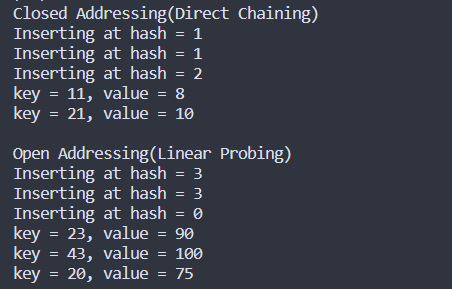
\includegraphics[]{Cycle_2/Outputs/Hashing.png}

\section{Result}
Hash table implemented using chaining method and linear probing. The program was
executed and output verified.
